\documentclass[a0,portrait]{a0poster}

\usepackage{multicol} % This is so we can have multiple columns of text side-by-side
\columnsep=100pt % This is the amount of white space between the columns in the poster
\columnseprule=3pt % This is the thickness of the black line between the columns in the poster

\usepackage[svgnames]{xcolor} % Specify colors by their 'svgnames', for a full list of all colors available see here: http://www.latextemplates.com/svgnames-colors

%\usepackage{times} % Use the times font
%\usepackage{palatino} % Uncomment to use the Palatino font
%\usepackage{tgheros}
\usepackage{helvet}
\renewcommand{\familydefault}{\sfdefault}

\usepackage{graphicx} % Required for including images
\graphicspath{{figures/}} % Location of the graphics files
\usepackage{booktabs} % Top and bottom rules for table
\usepackage[font=small,labelfont=bf]{caption} % Required for specifying captions to tables and figures
\usepackage{amsfonts, amsmath, amsthm, amssymb} % For math fonts, symbols and environments
\usepackage{wrapfig} % Allows wrapping text around tables and figures
\usepackage{blindtext}
\usepackage[numbers, sort, compress]{natbib}
\usepackage{float}
\usepackage{adjustbox}
\usepackage{setspace}
\usepackage{caption}
\usepackage[utf8]{inputenc}
\usepackage[spanish]{babel}
\usepackage{url}
\usepackage{listings}
\usepackage{subcaption}
\usepackage{hyperref}

\usepackage[explicit]{titlesec}
\usepackage{tikz}
    \usetikzlibrary{arrows, matrix, calc, shapes.geometric, shapes.misc,positioning}


%----------------------PREAMBLE-------------------------%
\setlength\parindent{0pt}

%------------------------HEADER-------------------------%

\begin{document}
\begin{minipage}[b]{0.20\linewidth}
    \begin{center}
        
\includegraphics[width=13cm]{uanl.eps}\\
        \vspace{5.5cm}
    \end{center}
\end{minipage}
%
\begin{minipage}[b]{0.60\linewidth}
    \begin{center}
        \veryHuge \color{Black} \textbf{Detección de melanoma de piel mediante segmentación semántica} \color{Black} \\[0.5cm]
        \Huge \textit{Redes Neuronales Convolucionales}\\[2cm]
        \LARGE \textbf{Mario Alberto Flores Hernández}\\[0.5cm]
        \huge UANL - FIME \\[0.5cm]
        \Large \texttt{mario.floreshe@uanl.edu.mx}
    \end{center}
\end{minipage}
%
\begin{minipage}[b]{0.20\linewidth}
    \begin{center}
        
\includegraphics[width=9cm]{fime.eps}\\
        \vspace{5cm}    
    \end{center}
\end{minipage}

\vspace{1cm}

%------------------------BODY---------------------------%
\begin{multicols}{3}
\large
\section*{Introducción}
El \textbf{melanoma de piel} es un tipo de cáncer maligno que se propaga rápidamente a otras partes del cuerpo mediante el fenómeno de metástasis incrementando rápidamente su probabilidad de mortalidad. Una forma de amortiguar los riesgos de esta enfermedad es mediante la detección temprana de su presencia.

La inteligencia artificial brinda soluciones para la resolución de problemas que involucran visión computacional, una tecnología reciente que ha demostrado ser muy versátil es la red neuronal convolucional.

La \textbf{segmentación semántica} es una técnica de clasificación en la que se obtiene un mapa probabilístico con las regiones categorizadas de una imagen entrante, como resultado de una secuencia de filtros y transformaciones.

\section*{Características Dimensionales}
Las imágenes a escala de grises y a color no comparten las mismas características dimensionales. Las imágenes a escala de grises se consideran un mapa bidimensional de intensidad de pixeles, mientras que las imágenes a color se consideran tridimensionales, siendo la tercera dimensión la capa de color.

\definecolor{red_matrix}{rgb}{0.6, 0, 0}
\definecolor{green_matrix}{rgb}{0, 0.8, 0}
\definecolor{blue_matrix}{rgb}{0, 0.25, 1}

\vspace{1cm}
\begin{center}
    \begin{tikzpicture}
        \draw[step=1cm, black, line width=0.80mm] (-5,-5) grid (5,5);
        \node at (0,-6) {$\text{dim} = m \times n$};
    \end{tikzpicture}
    \captionof{figure}{Imagen a escala de grises.}        
\end{center}
%
\begin{center}
    \begin{tikzpicture}
        \draw[step=1cm, red_matrix, line width=0.80mm] (-5,-5) grid (5,5);
        \draw[step=1cm, green_matrix, line width=0.80mm] (-4,-4) grid (6,6);
        \draw[step=1cm, blue_matrix, line width=0.80mm] (-3,-3) grid (7,7);
        \node at (0,-6) {$\text{dim} = m \times n \times k$};
    \end{tikzpicture}
    \captionof{figure}{Imagen a escala de grises.}        
\end{center}

\section*{Imágenes Dermatológicas}
Para entrenar un modelo de red neuronal convolucional de segmentación semántica es necesaria una base de datos que contenga dos subconjuntos: (a) imagen entrante, (b) salida deseada. La base de datos utilizada en esta implementación fue obtenida de la recopilación de imágenes dermatológicas internacional para la detección del melanoma \citep{isic_skin}.

\begin{center}
    \begin{tabular}{c c}
    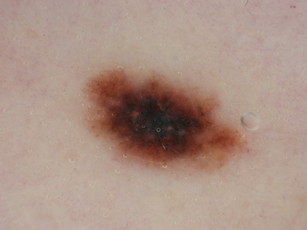
\includegraphics{input_1.png} &
    
\includegraphics{mask_1.png} \\
    (a) Imagen Entrante & (b) Máscara Computada\\         
    \end{tabular}
    \captionof{figure}{Comparación de la imagen dermatológica entrante y su respectiva máscara segmentada.}
\end{center}

\vspace{2cm}

%\begin{center}
%    
\includegraphics[scale=0.5]{mask_1.png}
%    \captionof{figure}{Imagen a escala de grises.}        
%\end{center}

\section*{Implementación}

El tipo de arquitectura utilizada para la implementación se denomina \texttt{FPN} o red piramidal de características, como encriptador se utilizó el arreglo de capas de convolución \texttt{RESNEXT}.
\begin{center}
    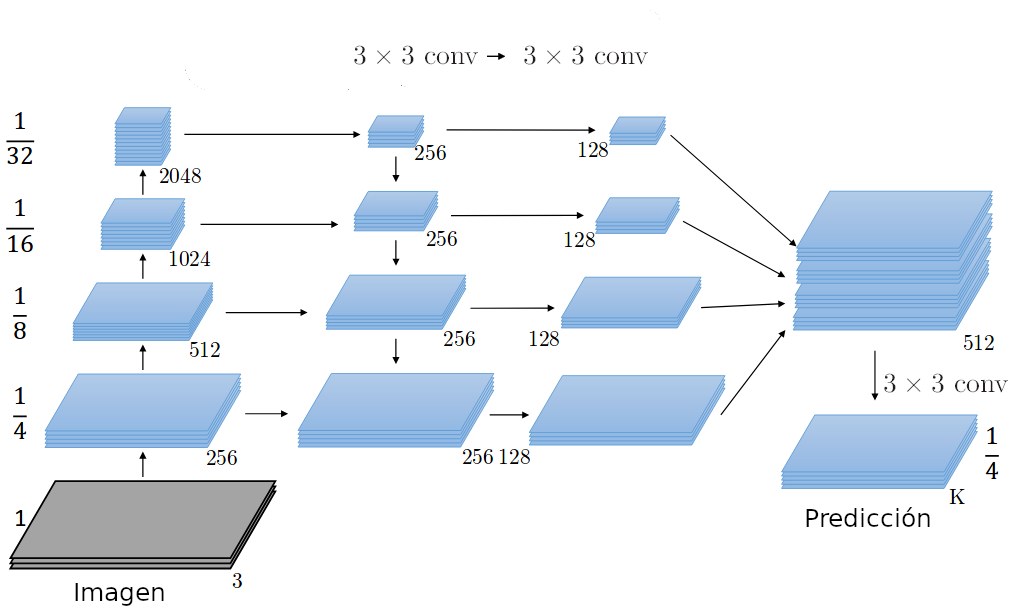
\includegraphics[scale=0.70]{fpn_ar_esp_2.png}
    \captionof{figure}{Representación de la arquitectura FPN \citep{fpn_2}.}
    \label{fig:fpn_map}
\end{center}

El lenguaje utilizado para la implementación de la arquitectura de la red neuronal convolucional fue \texttt{Python}, debido a que es un lenguaje dinámico y que contiene la librería de \texttt{Torch} la cual es requerida para la manipulación de los subconjuntos de datos y el entrenamiento de modelos.

\renewcommand{\lstlistingname}{Código}
\definecolor{codegreen}{rgb}{0,0.6,0}
\definecolor{codeblue}{rgb}{0.121, 0.203, 0.858}
\definecolor{codegray}{rgb}{0.5,0.5,0.5}
\definecolor{codepurple}{rgb}{0.58,0,0.82}
\definecolor{backcolour}{rgb}{0.95,0.95,0.92}

\lstdefinestyle{pystyle}{
    basicstyle= \normalsize\ttfamily\linespread{.8},
    backgroundcolor=\color{backcolour},   
    commentstyle=\color{codegreen},
    keywordstyle=\color{codeblue},
    numberstyle=\tiny\color{codegray},
    stringstyle=\color{codepurple},
    breakatwhitespace=false,         
    breaklines=true,                 
    captionpos=b,                    
    keepspaces=true,                 
    numbers=left,                    
    numbersep=5pt,                  
    showspaces=false,                
    showstringspaces=false,
    showtabs=false,                  
    tabsize=2
}

\lstset{style=pystyle}

\begin{lstlisting}[language = Python, label = {code:train} ,caption= Búcle de entrenamiento. ]
# train_model.py
max_score = 0 
for i in range(0,40):
    print('\n Epoch: {}'.format(i))
    train_logs = train_epoch.run(train_loader)
    valid_logs = valid_epoch.run(valid_loader)
    if max_score < valid_logs['iou_score']:
        max_score = valid_logs['iou_score']
        torch.save(model,('Model/'+encoder+'.pth'))
        print('Highest Score Model Saved: {}'.format(max_score))
\end{lstlisting}

\section*{Intensidad de Pixeles}
El \textbf{filtro de umbral} es un tipo de procesamiento de imágenes que discretiza los valores de intensidad dependiendo de un \textbf{coeficiente límite}. Si el valor del pixel se encuentra por debajo del coeficiente límite, se reduce a la intensidad mínima; por el contrario si el valor rebaza el coeficiente límite, se amplifica a la intensidad máxima.

\section*{Coeficiente de Dados}
El \textbf{coeficiente de dados} es una ecuación que determina el error entre dos matríces mediante la intersección de los pixeles coincidentes entre el total de pixeles. Este criterio es aplicado durante el proceso de entrenamiento.

\begin{center}
    \begin{equation}
        \text{CD} = \frac{2|A \cap B |}{|A| + |B|}
    \end{equation}        
\end{center}

\section*{Criterio de Jaccard}
El \textbf{criterio de Jaccard} es una ecuación muy similar al \textbf{coeficiente de dados}, la diferencia radíca en la penalización del error. El criterio de Jaccard penaliza aún más la diferencia entre las matríces y se utiliza en el proceso de validación.

\begin{equation}\label{eq:jacc}
    \text{CJ} = \frac{|A \cap B|}{| A \cup B |} = \frac{|A \cap B|}{|A| + |B| - |A \cap B|} \text{,}
\end{equation}

\section*{Resultados}
\captionof{table}{Resumen de resultados por época.}
\begin{center}\vspace{1cm}
    \adjustbox{width=0.5\columnwidth}{%
    \begin{tabular}{ccc}
    \toprule
    \textbf{Época} & \textbf{CD} & \textbf{CJ} \\
    \midrule
     1 & 0.2968 & 0.5616 \\
     2 & 0.2972 & 0.5546 \\
     3 & 0.2690 & 0.5879 \\
     4 & 0.2960 & 0.6389 \\
     5 & 0.2371 & 0.8415 \\
     6 & 0.0929 & 0.8626 \\
     7 & 0.0792 & 0.8626 \\
     8 & 0.0692 & 0.8798 \\
     9 & 0.0556 & 0.9017 \\
     10 & 0.0542 & 0.9039 \\
    \bottomrule
    \end{tabular}}
\end{center}\vspace{1cm}    

\section*{Conclusión}
Mediante los resultados obtenidos de los criterios de evaluación se puede observar un déficit en el error reportado por el coeficiente dados (CD) y un incremento en la similitud de acuerdo al criterio de Jaccard (CJ).

\section*{Trabajo a Futuro}
\begin{itemize}
    \item Implementar redes neuronales con segmentación semántica multi-categorica.
\end{itemize}

\section*{Repositorio de GitHub}
Mediante el siguiente \textbf{código QR} puedes acceder a la implementación del proyecto y los datos generados de los experimentos.
%\vspace{2cm}
\begin{center}
    
\includegraphics[scale=0.4]{repoqr.eps}
\end{center}
\small{
\url{https://github.com/Btrox148/semantic-segmentation-skin}
}

\section*{Referencias}

\small

\nocite{adam_opt}

\renewcommand\refname{\vskip -1cm}
\bibliographystyle{mighelnat}
\bibliography{MiBiblio}


\end{multicols}
\end{document}